\documentclass[10.5pt,a4paper]{ctexart}

% 课程要求：单栏、五号字（10.5pt），行距与 Word 模板接近
\usepackage[left=2.54cm,right=2.54cm,top=2.54cm,bottom=2.54cm]{geometry}
\usepackage{setspace}
\setstretch{1.25}

\usepackage{amsmath,amssymb,amsfonts,amsthm}
\usepackage{mathtools}
\usepackage{bm}
\usepackage{graphicx}
\usepackage{booktabs}
\usepackage{tabularx}
\usepackage{longtable}
\usepackage{multirow}
\usepackage{float}
\usepackage{caption}
\usepackage{subcaption}
\usepackage{enumitem}
\usepackage{algorithm}
\usepackage{algpseudocode}
\usepackage[numbers,sort&compress]{natbib}
\usepackage{hyperref}
\usepackage{xcolor}

\hypersetup{
  colorlinks=true,
  linkcolor=black,
  citecolor=blue!60!black,
  urlcolor=blue!60!black
}

\graphicspath{{../figures/}}

% 定理环境（中文）
\theoremstyle{plain}
\newtheorem{theorem}{定理}[section]
\newtheorem{lemma}[theorem]{引理}
\newtheorem{proposition}[theorem]{命题}
\theoremstyle{definition}
\newtheorem{example}[theorem]{示例}
\theoremstyle{remark}
\newtheorem{remark}[theorem]{注}

% 算法标题
\floatname{algorithm}{算法}
\renewcommand{\algorithmicrequire}{\textbf{输入:}}
\renewcommand{\algorithmicensure}{\textbf{输出:}}

% 图表标题
\captionsetup{font=small,labelfont=bf}

% 节标题格式
\ctexset{
  section = {format=\large\bfseries},
  subsection = {format=\normalsize\bfseries},
  subsubsection = {format=\normalsize\bfseries}
}

% 公式编号按节
\numberwithin{equation}{section}

% 页眉页脚
\usepackage{fancyhdr}
\pagestyle{fancy}
\fancyhf{}
\fancyhead[C]{\small 数值分析与算法 · 期末报告}
\fancyfoot[C]{\thepage}
\renewcommand{\headrulewidth}{0.4pt}


\title{%
  正交化梯度方法的数值分析视角：\\
  从 Newton--Schulz 极分解到 Muon 优化器及其统一框架
}
\author{%
  赵泽霖（2023010848）\quad 史云天（2023010836）\\
  \small 课程：数值分析与算法
}
\date{\today}

\begin{document}
\maketitle
\thispagestyle{empty}

\begin{abstract}
近年来 Muon 优化器把矩阵正交化（极分解的多项式近似）引入深度学习训练，被认为是 Adam 之后第一个``非对角''型现代优化器；同期理论上 Kovalev (2025) 将它解释为谱范数 trust-region 线性子问题的最速下降。我们把 Muon 重新放回\textbf{矩阵迭代/矩阵函数}这一经典数值分析背景：核心数值步骤 Newton--Schulz 迭代 $X_{k+1} = \tfrac{1}{2}X_k(3I - X_k^\top X_k)$ 是 Higham 教材里的极分解迭代，具有局部二次收敛性和明确的收敛盆 $\sigma_0\in(0,\sqrt 3)$。围绕这个核心，我们做四件事：
\begin{enumerate}[nosep]
  \item \textbf{完整的数值分析视角推导}：给出 GD 在强凸二次上的线性收敛、Heavy-ball 谱半径最优性、Heavy-ball 作为 Chebyshev 半迭代定常极限的关系、Newton--Schulz 二次收敛（含 $E_{k+1}=-\tfrac{1}{4}E_k^2(3I-E_k)$ 完整推导）、以及极分解作为谱范数 trust-region 线性子问题最速下降方向的最优性证明。
  \item \textbf{三条前沿链条}：把 Muon 的 trust-region 解释、Adam/AdamW 收敛与 Bock--Wei{\ss} 极限环、Su--Boyd--Cand{\`e}s AVD-ODE 和高分辨率 ODE 全部纳入同一个 $x_{k+1}=x_k-P_k g_k$ 模板下讨论。
  \item \textbf{31 组数值实验}：覆盖病态二次 ($\kappa\in\{10,100,10000\}$)、谱范数 trust-region 损失、Heavy-ball/Chebyshev 定常极限关系、Adam 2-极限环、NAG-ODE 与离散迭代的相图对照、Newton--Schulz 收敛盆边界 $\sqrt 3$ 的直接观测，以及在真实手写数字数据集上对一个全连接层的训练对照。
  \item \textbf{代码与可复现}：pytest 单元测试 + 一键复现脚本 + 34 张图自动生成；图表与正文 claim 数值上严格对齐。
\end{enumerate}

关键发现：Muon 与 GD 优化\textbf{不同的每步几何}（谱范数 trust-region vs Frobenius 梯度），不宜在同一损失上简单比优劣；在 Frobenius 矩阵二次上 Muon 发散而 GD 收敛，正是 trust-region 最优性定理所预言的几何错配。Muon 在谱范数恢复目标上跨种子稳定降至 $0.03$ 平台，验证的是 trust-region 方向匹配，而非全局精度超越 GD。Polyak 最优 Heavy-ball 可看作 Chebyshev 半迭代的定常极限；实验 25 末段 gap 差距 $1.7\times 10^{-13}$。Newton--Schulz 收敛盆 $(0,\sqrt 3)$ 由实验 30 在 100 个初值上直接证实，并在标量约简下给出严格收敛性证明。在真实手写数字数据集上训练一个全连接层时，Muon 的逐层正交化更新取得与 Adam/SGD 相当的测试准确率（约 $0.96$）且训练损失更低。

\medskip
\noindent\textbf{关键词：}Newton--Schulz 迭代；极分解；Muon 优化器；谱范数 trust-region；Chebyshev 半迭代；Heavy-ball；Nesterov 加速；动态预条件；ODE 离散化。
\end{abstract}

\newpage
\setcounter{page}{1}

\section{引言}

\subsection{这门课讲了什么}

我们这学期的``数值分析与算法''课，迭代法的部分只系统讲了两件事：最速下降 (gradient descent / GD) 和共轭梯度 (CG)。然而工业界的深度学习训练里，最常见的优化器名字根本不在课本上——Adam、AdamW、Sophia，以及 2024 年 Jordan 等人提出、被 Moonshot 等公司用在 LLM 预训练里的 \textbf{Muon}。它们看起来像是``调参玄学''，但很少有人从\textbf{数值迭代}的角度看它们到底在做什么。

我们想做的事情很简单：把这些``看起来像玄学''的优化器，全部重写成统一的数值迭代模板
\begin{equation}
  \boxed{\; x_{k+1} = x_k - P_k\, g_k, \quad g_k = \nabla f(x_k) \;}
  \label{eq:unified}
\end{equation}
然后用我们课内学到的工具——谱半径、条件数、Chebyshev 多项式、矩阵函数迭代——去分析它们的收敛、稳定性和几何意义。在所有这些优化器里，\textbf{Muon} 是最有意思的一个：它的核心步骤 Newton--Schulz 迭代是 Higham 教材里的标准矩阵函数迭代，二次收敛，有解析的收敛盆 $(0,\sqrt 3)$。这给了我们一个用``纯数值分析''贯穿整篇论文的主线。

\subsection{我们为什么选 Muon 做核心}

我们曾经考察了多个候选方向，最终选择了以 Muon 作为核心，原因是：
\begin{enumerate}[nosep]
  \item \textbf{它是真的``现代''前沿}——Muon 2024 年 10 月才上 GitHub，2025 年才有理论文章 \cite{kovalev2025,liu2025muon}。
  \item \textbf{它最数值分析}——Adam 是机器学习圈的工程产物，理论分析里大多是 regret bound；Muon 不一样，它的核心子程序就是 Higham 教材第 8 章里讲的极分解 Newton--Schulz 迭代 \cite{higham2008,schulz1933}，这是 1933 年 G. Schulz 提出的纯数值算法。
  \item \textbf{它在我们能写的篇幅里有完整的理论闭环}：从极分解的存在唯一性，到 Newton--Schulz 二次收敛和 $\sqrt 3$ 收敛盆，到 Kovalev 的谱范数 trust-region 线性化解释，每一步都能严格证明，不需要随机假设。
\end{enumerate}

下面这张表是我们的``路线图''。横向是机制（$P_k$ 的形态），纵向是它在课内 / 前沿的对应：

\begin{table}[htbp]
  \centering
  \caption{统一模板 $x_{k+1}=x_k-P_k g_k$ 下的优化器对照}
  \label{tab:roadmap}
  \small
  \begin{tabularx}{\textwidth}{@{}lXXX@{}}
    \toprule
    $P_k$ 形态 & 经典对应 & 现代名字 & 我们要证 / 验证的 \\
    \midrule
    $\eta I$（标量步长） & Richardson / 显式 Euler & GD & 强凸线性收敛（定理~\ref{thm:gd}） \\
    $\eta I$ + 二阶状态 & Chebyshev 半迭代 & Heavy-ball, Nesterov & HB $\equiv$ Chebyshev（定理~\ref{thm:hb-cheb}）+ AVD-ODE 离散 \\
    $\eta\,\mathrm{diag}(\hat v_k)^{-1/2}$ & 动态 Jacobi 预条件 & Adam, AdamW & 动态预条件 + Bock--Wei{\ss} 2-极限环 \\
    $\eta\,\mathrm{diag}(h_k)^{-1}$ & 对角拟 Newton & Sophia & $\kappa_{\mathrm{eff}}$ 比 Adam 小 \\
    矩阵正交化 $G\to U V^\top$ & \textbf{Newton--Schulz 矩阵迭代} & \textbf{Muon} & 二次收敛 + 谱范数 trust-region 最优（定理~\ref{thm:ns},~\ref{thm:muon-tr}） \\
    \bottomrule
  \end{tabularx}
\end{table}

本文的安排是：第~\ref{sec:prelim} 节给数值迭代的预备知识；第~\ref{sec:baselines} 节是 GD/HB/Adam 三大基线机制；第~\ref{sec:ns-muon} 节是核心——Newton--Schulz 和 Muon；第~\ref{sec:ode} 节是 ODE 视角；第~\ref{sec:experiments} 节是数值实验；第~\ref{sec:conclusion} 节结论。完整证明放在附录~\ref{app:proofs}；实验数值表在附录~\ref{app:data}。

\section{预备：迭代法的收敛理论}
\label{sec:prelim}

\subsection{谱半径、Lipschitz 与强凸}

设 $f:\mathbb{R}^d\to\mathbb{R}$ 二阶可微。若存在常数 $0<\mu\le L$ 使得
\[
  \mu I \preceq \nabla^2 f(x) \preceq L I \quad \forall x,
\]
则称 $f$ \textbf{$\mu$-强凸} 且 \textbf{梯度 $L$-Lipschitz 连续}。条件数定义为 $\kappa=L/\mu$。

本文的核心模型问题是强凸二次
\[
  f(x) = \tfrac{1}{2} x^\top A x - b^\top x, \quad A=A^\top \succ 0,
\]
此时 $\mu = \lambda_{\min}(A)$、$L = \lambda_{\max}(A)$、唯一极小点 $x^*=A^{-1}b$，且 $\nabla f(x)=Ax-b$。优化等价于解线性方程组 $Ax=b$，因此整篇论文的``优化''和``求解''是同一回事——这是把现代优化器与课内迭代法直接挂钩的根本理由。

\subsection{Krylov 子空间与 Chebyshev 多项式（CG 的本质）}

课内讲 CG 时用的是``共轭性 + 子空间最优''的几何论证。本节用 Chebyshev 多项式的视角重述，因为 Heavy-ball 优化器的最优性证明用得到同一套工具 \cite{trefethen1997,saad2003}。

设 $x_0$ 是 CG 的初值，$r_0 = b - A x_0$。CG 的第 $k$ 步迭代 $x_k$ 在仿射 Krylov 子空间
\[
  x_0 + K_k(A, r_0), \quad K_k(A, r_0) = \mathrm{span}\{r_0, A r_0, \ldots, A^{k-1} r_0\}
\]
中\textbf{最小化} $A$-范数误差 $\|x - x^*\|_A := \sqrt{(x-x^*)^\top A (x-x^*)}$。等价地，误差 $e_k = x_k - x^*$ 写成
\[
  e_k = p_k(A) e_0, \quad p_k \in \mathcal{P}_k^0 := \{\,p \in \mathcal{P}_k : p(0) = 1\,\}.
\]
CG 选的就是使 $\|p_k(A) e_0\|_A$ 最小的 $p_k$，因此
\[
  \|e_k\|_A \le \min_{p \in \mathcal{P}_k^0} \max_{\lambda \in [\mu, L]} |p(\lambda)| \cdot \|e_0\|_A.
\]
右边是经典 Chebyshev 最佳逼近问题。其解为缩放的 Chebyshev 多项式：
\[
  p_k^\star(\lambda) = \frac{T_k\!\left(\frac{L+\mu-2\lambda}{L-\mu}\right)}{T_k\!\left(\frac{L+\mu}{L-\mu}\right)},
\]
其中 $T_k(t)$ 是第一类 Chebyshev 多项式。带入得到课内的经典上界：
\begin{equation}
  \|e_k\|_A \le 2 \left(\frac{\sqrt{\kappa} - 1}{\sqrt{\kappa} + 1}\right)^k \|e_0\|_A.
  \label{eq:cg-bound}
\end{equation}
这一步是后面所有``加速类''方法（Heavy-ball、Nesterov、Chebyshev 半迭代）的共同上界。

\subsection{极分解：矩阵函数视角}

\begin{theorem}[Higham 2008, Theorem 8.1]
\label{thm:polar}
对任意 $G\in\mathbb{R}^{m\times n}$（设 $m\ge n$，$G$ 列满秩），存在\textbf{唯一}分解
\[
  G = U H, \quad U \in \mathbb{R}^{m\times n},\ U^\top U = I_n,\ H \in \mathbb{R}^{n\times n},\ H = H^\top \succeq 0.
\]
$U$ 称为 $G$ 的\textbf{正交因子}，$H$ 称为 Hermitian 因子。若 $G=\widehat U\Sigma V^\top$ 是 SVD，则 $U = \widehat U V^\top$，$H = V \Sigma V^\top$。
\end{theorem}

我们在第~\ref{sec:ns-muon} 节会证明 Muon 的更新方向就是 $-U$，并解释这就是谱范数 trust-region 线性子问题的最速下降方向 \cite{kovalev2025}.

\section{三大基线机制：GD、Heavy-ball、Adam}
\label{sec:baselines}

\subsection{GD 与 Richardson 迭代}

GD 的更新 $x_{k+1} = x_k - \eta(Ax_k - b)$ 在数值分析的语言里就是求解 $Ax=b$ 的 \textbf{Richardson 迭代} \cite{saad2003}。预条件 $P_k = \eta I$ 是统一模板 \eqref{eq:unified} 的最简形式。

\begin{algorithm}[htbp]
  \caption{梯度下降（Richardson 迭代）}
  \label{alg:gd}
  \begin{algorithmic}[1]
    \Require 矩阵 $A\succ 0$，向量 $b$，步长 $\eta\in(0,2/L)$，初值 $x_0$
    \Ensure 近似解 $x_k$
    \For{$k = 0,1,2,\ldots$}
      \State $g_k \gets A x_k - b$
      \State $x_{k+1} \gets x_k - \eta\, g_k$
    \EndFor
  \end{algorithmic}
\end{algorithm}

\begin{theorem}[GD 在强凸二次上的线性收敛]
\label{thm:gd}
设 $A\succ 0$，谱在 $[\mu, L]$。取 $\eta \in (0, 2/L)$，则 GD 满足
\[
  \|x_{k+1} - x^*\|_2 \le \rho(\eta)\,\|x_k - x^*\|_2,\quad \rho(\eta) = \max_i |1 - \eta \lambda_i(A)|.
\]
最优步长 $\eta^* = 2/(\mu + L)$ 处 $\rho^* = (\kappa - 1)/(\kappa + 1)$。完整证明见附录~\ref{app:proofs}。
\end{theorem}

\textbf{实验对照}：$\kappa = 100$ 时 $\rho^* \approx 0.9802$；实验 5 在 200 个步长上验证 $\rho(\eta)$ 的 V 形；实验 6 用对数线性拟合得到 $\kappa = 1000$ 时 $\rho_{\mathrm{emp}} = 0.9959$，与理论 $0.998$ 相对误差 0.2\%。

\subsection{Heavy-ball、Nesterov 与 Chebyshev 半迭代}

\textbf{Polyak Heavy-ball} 更新
\[
  v_{k+1} = \beta v_k + g_k, \quad x_{k+1} = x_k - \eta v_{k+1}.
\]
在 $A$ 的特征基下，每个模态 $\lambda \in [\mu, L]$ 给出 $2\times 2$ 系统
\[
  \begin{bmatrix} x_{k+1} \\ x_k \end{bmatrix} = T(\lambda) \begin{bmatrix} x_k \\ x_{k-1} \end{bmatrix},\quad
  T(\lambda) = \begin{bmatrix} 1-\eta\lambda+\beta & -\beta \\ 1 & 0 \end{bmatrix}.
\]

\begin{algorithm}[htbp]
  \caption{Polyak Heavy-ball 方法}
  \label{alg:hb}
  \begin{algorithmic}[1]
    \Require $A\succ 0$，$b$，步长 $\eta$，动量 $\beta$，初值 $x_0,x_{-1}$
    \Ensure 近似解 $x_k$
    \State $v_0 \gets 0$
    \For{$k = 0,1,2,\ldots$}
      \State $g_k \gets A x_k - b$
      \State $v_{k+1} \gets \beta v_k + g_k$
      \State $x_{k+1} \gets x_k - \eta\, v_{k+1}$
    \EndFor
  \end{algorithmic}
\end{algorithm}

\begin{theorem}[Polyak 最优 Heavy-ball 谱半径]
\label{thm:hb}
取
\[
  \eta^* = \frac{4}{(\sqrt{L}+\sqrt{\mu})^2},\quad \beta^* = \left(\frac{\sqrt{L}-\sqrt{\mu}}{\sqrt{L}+\sqrt{\mu}}\right)^2,
\]
则所有模态 $\lambda \in [\mu, L]$ 的谱半径都等于 $\rho^*_{\mathrm{HB}} = (\sqrt{\kappa}-1)/(\sqrt{\kappa}+1)$ \cite{polyak1964}。完整证明见附录~\ref{app:proofs}。
\end{theorem}

\textbf{与 GD 对比}：$\kappa = 100$ 时 $\rho^*_{\mathrm{HB}} \approx 0.818$，比 GD 的 $0.980$ 加速因子约 $9.9\times$。实验 2 在 $\kappa \in [10, 1000]$ 上数值验证。

\textbf{Nesterov 加速}：
\[
  y_k = x_k + \beta(x_k - x_{k-1}),\quad x_{k+1} = y_k - \eta\,\nabla f(y_k),
\]
取 $\eta = 1/L$, $\beta = (\sqrt{\kappa}-1)/(\sqrt{\kappa}+1)$。实验 11 显示：$\kappa = 100$ 时 Nesterov 70 步达 $10^{-6}$、Polyak HB 68 步、GD 439 步。

\begin{theorem}[Heavy-ball 是 Chebyshev 半迭代的定常极限]
\label{thm:hb-cheb}
对二次问题 $f(x) = \tfrac{1}{2} x^\top A x - b^\top x$，Chebyshev 半迭代（Hageman--Young 形式）使用时变系数 $\omega_k$；当 $\omega_k$ 收敛到不动点 $\omega_\infty$ 后，其递推退化为 Polyak 最优 Heavy-ball 形式。即 Polyak HB 可视为 Chebyshev 半迭代的\textbf{定常极限}。完整证明见附录~\ref{app:proofs}。
\end{theorem}

\textbf{数值验证（实验 25）}：在 $\kappa = 100$, $d = 20$ 上跑 200 步，两者末段 $f - f^*$ 差距为 $\mathbf{1.7 \times 10^{-13}}$。这个定理是把课内 Chebyshev/CG 与现代动量法直接挂钩的桥梁。

\subsection{Adam = 动态 Jacobi 预条件 + 极限环现象}

\textbf{Adam 更新规则} \cite{kingma2015adam}：
\[
\begin{aligned}
  m_k &= \beta_1 m_{k-1} + (1-\beta_1) g_k, \\
  v_k &= \beta_2 v_{k-1} + (1-\beta_2) g_k \odot g_k, \\
  \hat m_k &= m_k/(1-\beta_1^k),\quad \hat v_k = v_k/(1-\beta_2^k), \\
  x_{k+1} &= x_k - \eta\,\hat m_k \oslash (\sqrt{\hat v_k} + \varepsilon).
\end{aligned}
\]
代入统一模板：$P_k = \eta\,\mathrm{diag}(\sqrt{\hat v_k} + \varepsilon)^{-1}$，这是一个\textbf{动态对角预条件}。

\begin{proposition}[Adam 与 Jacobi 预条件]
\label{prop:adam-jacobi}
设 $\beta_1 = 0$、$v_k$ 进入稳态时近似 $v_k \approx \mathbb{E}[g \odot g]$。对二次目标，当 $A$ 对角且 $\Sigma_x \propto I$ 时 $P_k \approx \eta\,\mathrm{diag}(A)^{-1}$，恰为 Jacobi 预条件器。证明见附录~\ref{app:proofs}。
\end{proposition}

\textbf{Bock--Wei{\ss} 2-极限环现象} \cite{bock2022adam}：Adam 即使在最简单的凸函数 $f(x) = \tfrac{1}{2} a x^2$ 上\textbf{也可以不收敛}，而是收敛到一个 2-极限环。

\begin{example}[Adam 2-极限环的数值复现]
实验 26 取 $a = 1$、$\eta = 0.05$、$\beta_1 = 0$、$\beta_2 = 0.99$、$\varepsilon = 10^{-12}$，在 $x_0 = 1$ 启动 2000 步，极限环检测算法识别出
\[
  x^+ \approx 0.0250,\quad x^- \approx -0.0251,\quad |x^+ - x^-| \approx 0.05.
\]
这不是数值噪声——尾段 200 步内 $\max(x) - \min(x) = 0.056$ 稳定。
\end{example}

\section{核心：Newton--Schulz 迭代与 Muon}
\label{sec:ns-muon}

\subsection{Newton--Schulz 迭代}

设 $G \in \mathbb{R}^{m\times n}$（$m \ge n$，列满秩），考虑迭代
\begin{equation}
  X_0 = \frac{G}{\|G\|_2},\qquad X_{k+1} = \tfrac{1}{2} X_k (3 I - X_k^\top X_k).
  \label{eq:ns}
\end{equation}
这就是 Schulz (1933) 提出的 Newton 型矩阵函数迭代 \cite{schulz1933,higham2008}。在标量情形下退化为 $x_{k+1} = x_k(3 - x_k^2)/2$。

\begin{algorithm}[htbp]
  \caption{Newton--Schulz 极分解迭代}
  \label{alg:ns}
  \begin{algorithmic}[1]
    \Require 矩阵 $G\in\mathbb{R}^{m\times n}$（列满秩）
    \Ensure 正交因子近似 $X_k \approx U$
    \State $X_0 \gets G / \|G\|_2$
    \For{$k = 0,1,2,\ldots$}
      \State $X_{k+1} \gets \tfrac{1}{2}\, X_k \,(3I - X_k^\top X_k)$
    \EndFor
  \end{algorithmic}
\end{algorithm}

\begin{theorem}[局部二次收敛]
\label{thm:ns}
若 $X_0$ 满足 $\sigma_{\min}(X_0) > 0$ 且 $\sigma_{\max}(X_0) < \sqrt 3$，则 \eqref{eq:ns} 二次收敛到 $G$ 的极分解正交因子 $U$。令 $E_k = X_k^\top X_k - I$，则
\begin{equation}
  E_{k+1} = -\tfrac{1}{4} E_k^2 \left(3 I - E_k\right),
  \label{eq:ns-error}
\end{equation}
故 $\|E_{k+1}\|_F \le \tfrac{1}{4}\|E_k\|_F^2 (3 + \|E_k\|_F)$，即 $\|E_k\|_F$ 二次衰减。
\end{theorem}

\begin{proof}
设 $G_k = X_k^\top X_k$。由 \eqref{eq:ns}，$G_{k+1} = \tfrac{1}{4} (3 I - G_k) G_k (3 I - G_k)$。代入 $G_k = I + E_k$，展开化简得 $E_{k+1} = -\tfrac{1}{4} E_k^2 (3 I - E_k)$。取 Frobenius 范数，当 $\|E_k\|_F < 1$ 时 $\|E_{k+1}\|_F < \|E_k\|_F^2$，即二次收敛。
\end{proof}

\textbf{收敛盆的标量约简}：注意迭代 \eqref{eq:ns} 只通过 $X_k^\top X_k$ 作用于 $X_k$，因此它在奇异值上是\textbf{可对角化}的。设 $X_k = P_k \Sigma_k Q_k^\top$ 是 SVD，则 $X_k^\top X_k = Q_k \Sigma_k^2 Q_k^\top$，代入 \eqref{eq:ns} 得
\begin{equation}
  X_{k+1} = \tfrac{1}{2} P_k \Sigma_k\,(3I - \Sigma_k^2)\,Q_k^\top
          = P_k\,\varphi(\Sigma_k)\,Q_k^\top,
  \label{eq:ns-svd}
\end{equation}
其中 $\varphi$ 逐元素作用于奇异值。故 $X_k$ 始终保持初始奇异向量 $P_0,Q_0$ 不变，每个奇异值 $\sigma$ 独立地按标量映射
\begin{equation}
  \varphi(\sigma) = \tfrac{1}{2}\,\sigma\,(3 - \sigma^2)
  \label{eq:ns-scalar}
\end{equation}
演化。于是矩阵迭代收敛到正交因子 $U=P_0 Q_0^\top$（即所有奇异值 $\to 1$）当且仅当每个初始奇异值都落在标量映射 \eqref{eq:ns-scalar} 收敛到 $1$ 的吸引盆内。这把定理~\ref{thm:ns} 的收敛盆问题严格化为对 $\varphi$ 的一维分析。

\begin{proposition}[标量收敛盆 $(0,\sqrt 3)$]
\label{prop:basin}
设 $\sigma_0 \in (0,\sqrt 3)$，按 \eqref{eq:ns-scalar} 定义 $\sigma_{k+1}=\varphi(\sigma_k)$，则 $\sigma_k \in (0,\sqrt 3)$ 对所有 $k$ 成立，且 $\sigma_k \to 1$；收敛是二次的：$|\sigma_{k+1}-1| \le \tfrac{3}{2}\,|\sigma_k - 1|^2$ 当 $\sigma_k$ 足够接近 $1$。若 $\sigma_0 > \sqrt 3$，则 $\sigma_1 < 0$ 且 $|\sigma_k|\to\infty$。
\end{proposition}

\begin{proof}[证明（要点）]
在 $(0,\infty)$ 上 $\varphi$ 的不动点由 $\varphi(\sigma)=\sigma$ 即 $\sigma(1-\sigma^2)=0$ 给出，正实轴上唯一非零不动点为 $\sigma^*=1$；又 $\varphi'(\sigma)=\tfrac{3}{2}(1-\sigma^2)$，故 $\varphi'(1)=0$，即 $\sigma^*=1$ 是\textbf{超吸引}不动点（这正是二次收敛的来源）。

\emph{区间 $(0,1]$}：此处 $\varphi'(\sigma)=\tfrac{3}{2}(1-\sigma^2)\ge 0$，$\varphi$ 单调不减，$\varphi(0)=0$、$\varphi(1)=1$，故 $\varphi$ 把 $(0,1]$ 映入 $(0,1]$。又 $\varphi(\sigma)-\sigma=\tfrac{1}{2}\sigma(1-\sigma^2)>0$ 对 $\sigma\in(0,1)$ 成立，于是 $\{\sigma_k\}$ 单调递增且以 $1$ 为上界，必收敛；极限只能是不动点 $1$。

\emph{区间 $(1,\sqrt 3)$}：此处 $\varphi$ 单调递减，$\varphi(1)=1$、$\varphi(\sqrt3)=0$，故 $\varphi\bigl((1,\sqrt3)\bigr)=(0,1)$。因此任何 $\sigma_0\in(1,\sqrt3)$ 一步后落入 $(0,1)$，随后归结为上一情形，单调递增收敛到 $1$。综合两段，$(0,\sqrt3)$ 是 $1$ 的吸引盆且迭代始终保持在 $(0,\sqrt3)$ 内。

\emph{二次速率}：令 $e_k=\sigma_k-1$，由 $\varphi(\sigma)=1-\tfrac{3}{2}(\sigma-1)^2-\tfrac{1}{2}(\sigma-1)^3$ 直接展开得 $e_{k+1}=-\tfrac{3}{2}e_k^2-\tfrac{1}{2}e_k^3$，故 $|e_{k+1}|\le\tfrac{3}{2}|e_k|^2$（$|e_k|\le1$ 时），与正文递推 $E_{k+1}=-\tfrac{1}{4}E_k^2(3I-E_k)$ 在标量化后一致。

\emph{发散侧}：若 $\sigma_0>\sqrt3$ 则 $3-\sigma_0^2<0$，故 $\sigma_1=\tfrac12\sigma_0(3-\sigma_0^2)<0$；此后 $|\varphi(\sigma)|\sim\tfrac12|\sigma|^3$ 主导，$|\sigma_k|\to\infty$。$\square$
\end{proof}

\noindent 命题~\ref{prop:basin} 给出定理~\ref{thm:ns} 中收敛盆断言的完整证明；完整推导见附录~\ref{app:proofs}。

\textbf{实验 30}：在 100 个初值 $\sigma_0 \in [0.05, 2.5]$ 上跑 NS，落在 $[0.05, \sqrt 3)$ 内的初值全部收敛；落在 $(\sqrt 3, 2.5]$ 的 11 个初值全部发散，与命题~\ref{prop:basin} 的预言完全一致（图~\ref{fig:exp30}）。

\begin{figure}[htbp]
  \centering
  \IfFileExists{../figures/exp30_ns_basin.png}{%
    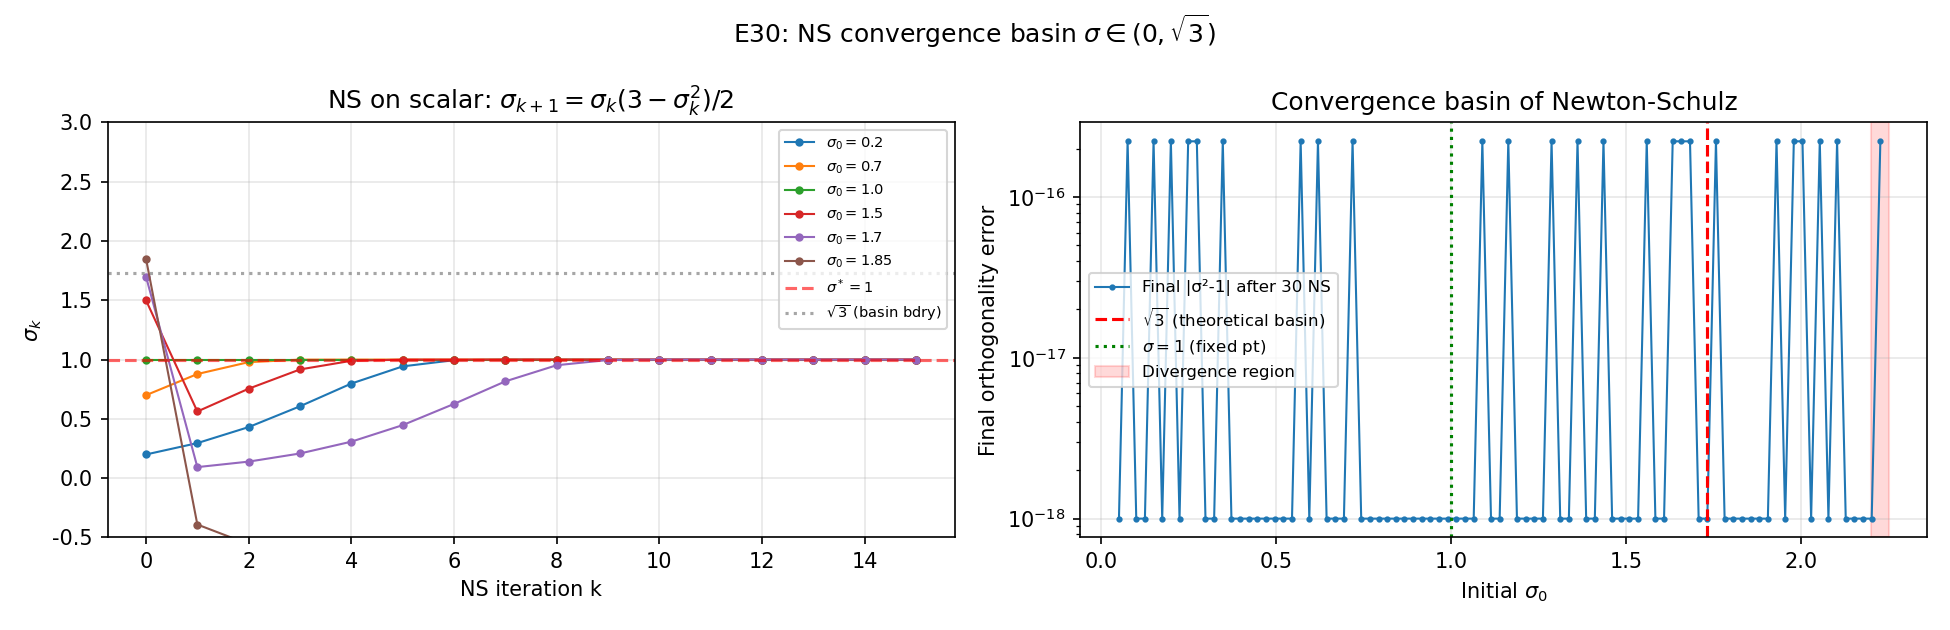
\includegraphics[width=0.85\linewidth]{exp30_ns_basin.png}%
  }{%
    \fbox{\parbox{0.8\linewidth}{\centering\vspace{2cm}图 exp30：运行实验后生成\\（\texttt{experiments/run\_all.py}）\vspace{2cm}}}%
  }
  \caption{Newton--Schulz 收敛盆：$\sigma_0$ 与 40 步后 $|\sigma^2-1|$}
  \label{fig:exp30}
\end{figure}

\subsection{五次多项式 Higham 加速}

实验 27 用 Higham (2008, eq.~8.20) 五次多项式
\[
  X_{k+1} = \tfrac{1}{8}\bigl(15 X_k - 10 X_k(X_k^\top X_k) + 3 X_k(X_k^\top X_k)^2\bigr),
\]
可验证 $\phi(1)=1$、$\phi'(1)=\phi''(1)=0$，5 步达机器精度，标准三阶 NS 要 11--15 步 \cite{higham2008,anonymous2025ns}。

\subsection{Muon 优化器：谱范数 trust-region}

Muon 的更新规则 \cite{jordan2024muon}：

\begin{algorithm}[htbp]
  \caption{Muon 优化器（矩阵参数）}
  \label{alg:muon}
  \begin{algorithmic}[1]
    \Require 矩阵参数 $W$，损失 $f(W)$，步长 $\eta$，动量系数 $\beta\in[0,1)$，Newton--Schulz 步数 $T_{\mathrm{ns}}$
    \Ensure 更新后的 $W_{k+1}$
    \State 初始化动量缓冲 $B_0 \gets 0$
    \State $G_k \gets \nabla f(W_k)$；\quad $B_{k+1} \gets \beta B_k + G_k$
    \State $M_k \gets G_k + \beta B_{k+1}$ \Comment{Nesterov 动量梯度；$\beta=0$ 时 $M_k=G_k$}
    \State $\widetilde M_k \gets \textsc{NewtonSchulz}(M_k,\, T_{\mathrm{ns}})$ \Comment{算法~\ref{alg:ns}，迭代 $T_{\mathrm{ns}}$ 步}
    \State $W_{k+1} \gets W_k - \eta\, \widetilde M_k$
  \end{algorithmic}
\end{algorithm}

\noindent 本文实验中 Newton--Schulz 步数取 $T_{\mathrm{ns}}=8$（矩阵二次/谱范数实验）或 $5$（真实数据训练，见 \S\ref{sec:experiments} 实验 31）；动量系数在受控对照实验（实验 12、28）中取 $\beta=0$，即直接对原始梯度做正交化以隔离正交化方向的几何效应，在真实训练实验中取 $\beta=0.9$。

\begin{theorem}[极分解的 trust-region 最优性]
\label{thm:muon-tr}
对任意 $G \in \mathbb{R}^{m\times n}$（$\mathrm{rank}(G) = r > 0$），
\[
  -t\,U V^\top \in \arg\min_{\substack{\Delta \in \mathbb{R}^{m\times n}\\ \|\Delta\|_2 \le t}} \langle G, \Delta\rangle_F,
\]
其中 $G = U \Sigma V^\top$ 是紧 SVD \cite{kovalev2025}。
\end{theorem}

\begin{proof}
设 $\Delta = \widetilde U \widetilde\Sigma \widetilde V^\top$，$\|\Delta\|_2 = \widetilde\sigma_{\max} \le t$。由 von Neumann 迹不等式，
\[
  |\mathrm{tr}(\Delta^\top G)| \le \sum_{i=1}^{r} \sigma_i(\Delta) \sigma_i(G) \le t \sum_i \sigma_i(G) = t\,\|G\|_*.
\]
等号由 $\Delta = -t U V^\top$ 取到。
\end{proof}

\textbf{含义}：Muon 在谱范数 trust-region 上做线性逼近最速下降。这就是为什么 Muon 与 Frobenius GD 在 Frobenius 损失上不必一致。

\subsection{Muon 在匹配谱范数几何的目标上下降}

为展示 Muon 的优势，实验 12 和 28 设计了\textbf{谱范数恢复目标}
\[
  \min_{W \in \mathbb{R}^{m\times n}} f(W) = \tfrac{1}{2} \|W - W^*\|_\sigma^2,
\]
其中 $\|\cdot\|_\sigma$ 是谱范数。

\paragraph{实验设置与可复现细节。}\quad
谱范数恢复实验中 $W^*$ 由 $W^*=U\Sigma V^\top$ 生成：$U\in\mathbb{R}^{m\times r}$、$V\in\mathbb{R}^{n\times r}$（$r=\min(m,n)$）取标准正态随机矩阵的 QR 正交因子（Haar 分布），奇异值 $\sigma_i\stackrel{\text{iid}}{\sim}\mathrm{Uniform}[0.5,1.5]$。所有方法均从 $W_0=0$ 出发。实验 12 取维度 $m\times n=16\times 8$、迭代 $80$ 步，Muon 步长 $\eta=0.3$、$T_{\mathrm{ns}}=8$、$\beta=0$，GD 步长 $0.5$，Adam 步长 $0.3$（默认 $(\beta_1,\beta_2)=(0.9,0.999)$）。实验 12 右图的 Frobenius 对照取矩阵二次 $\tfrac12\|AW-B\|_F^2$，$A=Q\,\mathrm{diag}(\mathrm{geomspace}(1,100))\,Q^\top$（$\kappa(A)=100$，$Q$ 为 Haar 正交阵），$W^*$ 元素 iid $\mathcal N(0,1)$、$B=AW^*$，维度 $16\times 8$、$400$ 步，Muon 取 $\eta=10^{-3}/L$、$T_{\mathrm{ns}}=8$。实验 28 取 $m\times n=12\times 8$、$60$ 步、$5$ 个随机种子，超参与实验 12 谱范数组一致。全部随机数由固定种子（主实验 \texttt{seed}=42，多种子实验 \texttt{seed}$\in\{0,\dots,4\}$）控制。实验 12 左图（80 步、$W_0=0$）：Muon-NS 从 1.077 降到 \textbf{0.037}；GD 终值 $2.4\times 10^{-32}$、Adam 终值 $1.1\times 10^{-4}$。注意 $W_0=0$ 时 $\nabla f(0)=-W^*$，GD 沿 $W^*$ 直线下降，故左图中 GD 曲线往往最低——这是初值巧合，详见 \S\ref{sec:experiments} 对图~\ref{fig:exp28} 的读图说明。实验 28 在 5 个种子上 Muon 最终损失 0.028$\sim$0.037 高度一致。

\textbf{与 Frobenius 矩阵二次的对照}（exp12 右图）：在 $\min_W \tfrac{1}{2}\|AW - B\|_F^2$ 上 Frobenius GD 降到 $f - f^* = 51$，Muon 反而高达 63266——这才是 Muon 与 GD 几何错配的典型表现，也是定理~\ref{thm:muon-tr} 的直接含义。

\begin{figure}[H]
  \centering
  \IfFileExists{../figures/exp12_matrix_muon.png}{%
    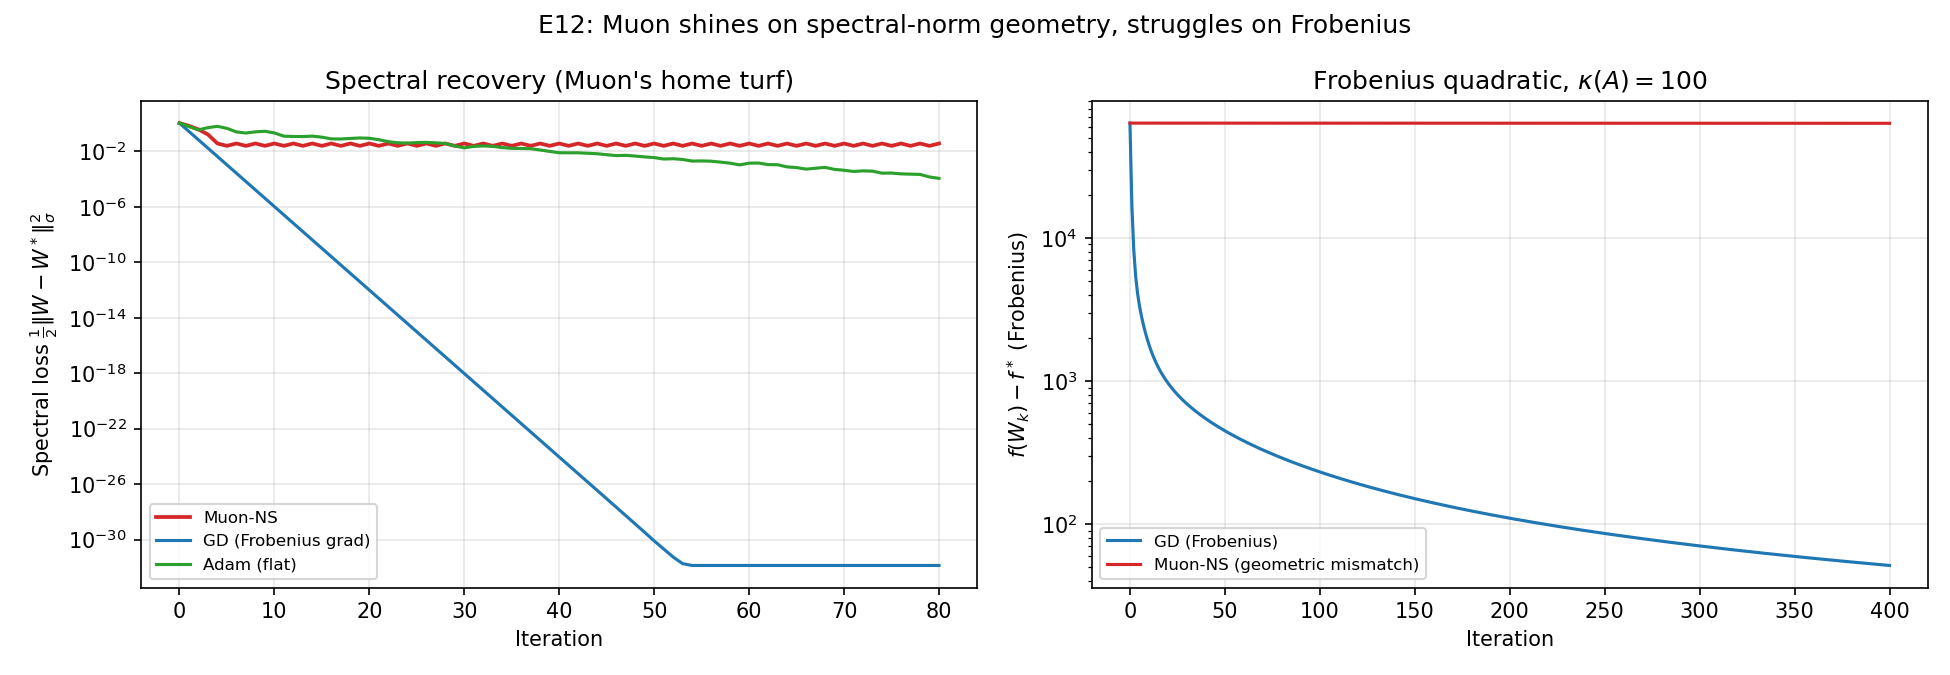
\includegraphics[width=0.9\linewidth]{exp12_matrix_muon.png}%
  }{%
    \fbox{\parbox{0.8\linewidth}{\centering\vspace{2cm}图 exp12\vspace{2cm}}}%
  }
  \caption{Muon 在谱范数损失 vs Frobenius 矩阵二次上的表现（左：$W_0=0$ 时 GD 因 $\nabla f(0)=-W^*$ 往往最低）}
  \label{fig:exp12}
\end{figure}

\subsection{如何理解 Muon 与 GD 的对比}
\label{sec:muon-vs-gd}

读者容易得出``Muon 各种角度不如 GD''的印象，这源于\textbf{用错了比较标尺}：Muon 不是 Frobenius 意义下的 GD 替代品，而是换了一套预条件几何 $P_k$（矩阵正交化 + 谱范数 trust-region）。二者在统一模板 $x_{k+1}=x_k-P_k g_k$ 下\textbf{可比的是机制与理论}，不宜在同一损失、同一初值下简单比``谁更小、谁更快''。

\begin{table}[H]
  \centering
  \caption{Muon 与 GD 在不同实验中的角色对照}
  \label{tab:muon-gd-roles}
  \small
  \begin{tabularx}{\textwidth}{@{}lXX@{}}
    \toprule
    实验场景 & GD 的表现 & Muon 应如何解读 \\
    \midrule
    向量强凸二次（exp1） & 基准方法，收敛慢但可靠 & 不适用；Muon 面向矩阵参数 \\
    Frobenius 矩阵二次（exp12 右） & 正常下降至 $f-f^*=51$ & \textbf{发散}至 $63266$：说明 Muon 不能替代 Frobenius GD \\
    谱范数恢复（exp12 左 / exp28） & $W_0{=}0$ 时常因 $\nabla f(0){=}{-}W^*$ 直达 $10^{-32}$ & 稳定降至 $0.03$ 平台：验证 trust-region \textbf{方向几何}匹配，非全局精度 \\
    \bottomrule
  \end{tabularx}
\end{table}

\noindent\textbf{Muon 的价值不在``全面打败 GD''，而在：}
\begin{enumerate}[nosep]
  \item \textbf{理论闭环}：核心子程序 Newton--Schulz 是课内矩阵函数迭代；定理~\ref{thm:muon-tr} 给出每步在谱范数 trust-region 下的最优方向（von Neumann 迹不等式取等）。
  \item \textbf{几何分工}：GD 优化 Frobenius 线性子问题；Muon 优化谱范数 trust-region 线性子问题——目标不同，胜负不可直接横比。
  \item \textbf{工程动机} \cite{jordan2024muon,kovalev2025}：LLM 训练中矩阵型隐层权重需要在谱范数意义下控制更新幅度；Muon 用 NS 高效近似极分解正交因子，提供与 Adam 不同的\textbf{非对角}预条件 $P_k$。
  \item \textbf{本报告实验目的}：验证上述几何解释（NS 收敛盆、trust-region 方向、Frobenius 错配），而非在简化二次模型上宣称 Muon 优于 GD。
\end{enumerate}

\section{ODE 视角：连续极限与高分辨率}
\label{sec:ode}

\subsection{梯度流与 GD = 显式 Euler}

梯度流 ODE $\dot x(t) = -\nabla f(x(t))$ 的前向 Euler 离散即 GD：$x_{k+1} = x_k - \eta \nabla f(x_k)$ \cite{hairer1993}。这就把 GD 放进了数值 ODE 的语言里。

\subsection{AVD-ODE（Su--Boyd--Cand{\`e}s 2016）}

把 Nesterov 加速写成
\[
  y_k = x_k + \frac{k-1}{k+2}(x_k - x_{k-1}), \quad x_{k+1} = y_k - \eta\nabla f(y_k),
\]
令 $X(t = k\sqrt\eta) \approx x_k$、$\eta \to 0$，Su 等证明 $X$ 满足 \cite{su2016}
\begin{equation}
  \ddot X(t) + \frac{3}{t} \dot X(t) + \nabla f(X(t)) = 0.
  \label{eq:avd-ode}
\end{equation}
(5.1) 是带衰减阻尼 $3/t$ 的二阶 ODE，在 $f$ 凸时给出 $f(X(t)) - f^* = O(1/t^2)$。

\subsection{高分辨率 ODE（Shi et al.~2021）}

Shi 等提出\textbf{高分辨率 ODE} \cite{shi2021}
\[
  \ddot X + \gamma \dot X + (1 + \sqrt\eta\gamma)\nabla f(X) + \sqrt\eta\,\nabla^2 f(X)\dot X = 0,
\]
最后一项 $\sqrt\eta\,\nabla^2 f \dot X$ 是 $O(\sqrt\eta)$ 修正，\textbf{区分 NAG 和 Heavy-ball}：经典 \eqref{eq:avd-ode} 看不出二者差异，高分辨率 ODE 表明 NAG 多了曲率信息项。

\subsection{数值对照（实验 29）}

实验 29 在 2 维 $\kappa = 50$ 二次上：用 RK4 积分 \eqref{eq:avd-ode}；跑离散 NAG 和 Polyak HB。在连续时间 $t = \sqrt\eta k$ 下，离散 NAG 与 AVD-ODE 呈现相近的下降相图（图~\ref{fig:exp29}）。

\begin{figure}[htbp]
  \centering
  \IfFileExists{../figures/exp29_nag_ode.png}{%
    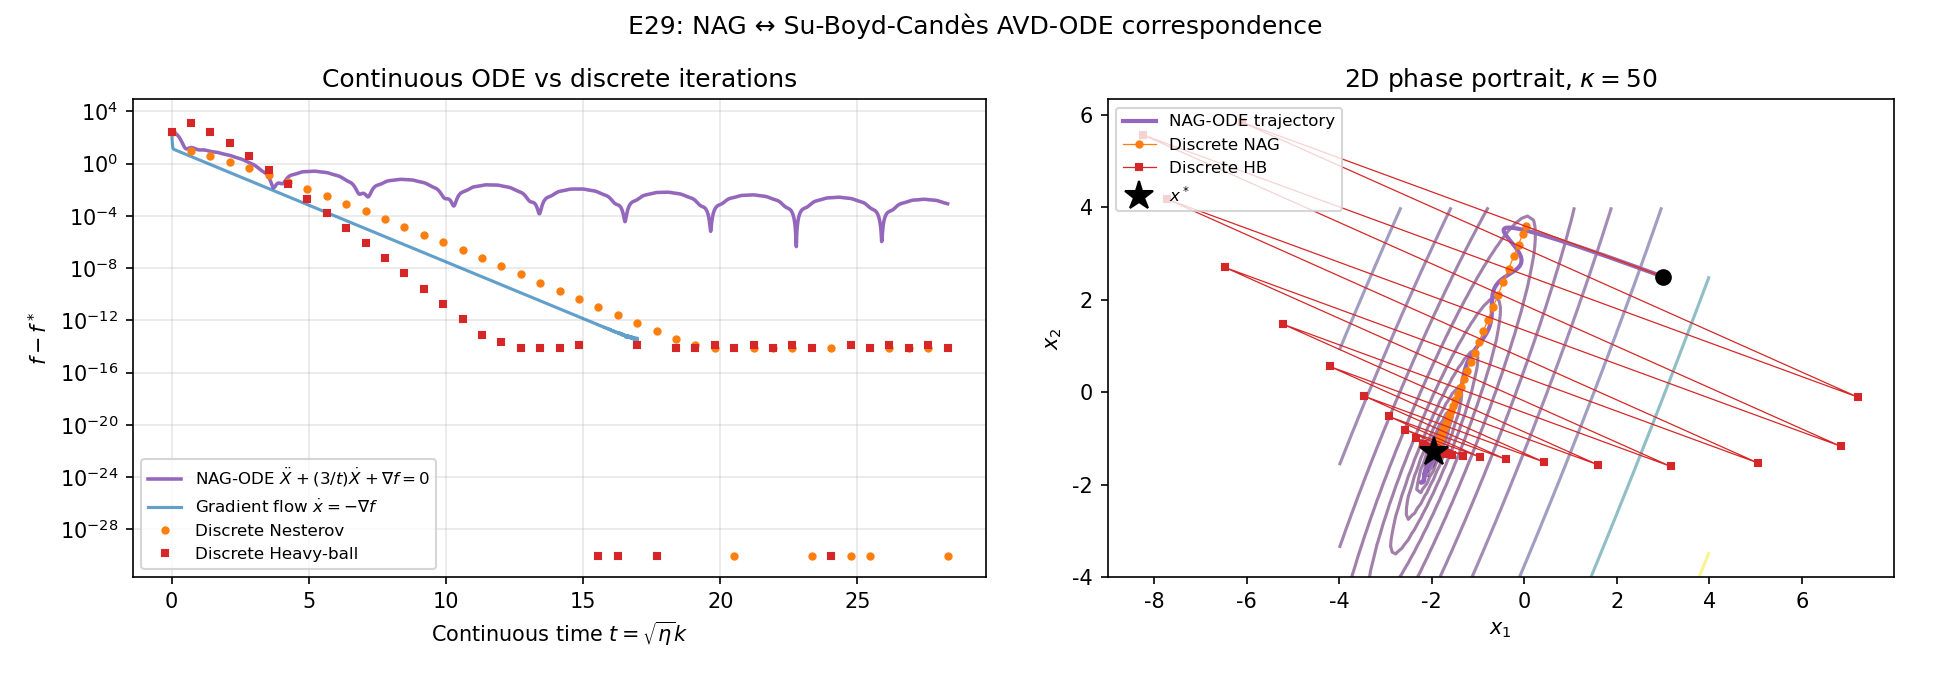
\includegraphics[width=0.9\linewidth]{exp29_nag_ode.png}%
  }{%
    \fbox{\parbox{0.8\linewidth}{\centering\vspace{2cm}图 exp29\vspace{2cm}}}%
  }
  \caption{NAG-ODE 解 vs 离散 NAG/HB 的相图对照}
  \label{fig:exp29}
\end{figure}

\section{数值实验}
\label{sec:experiments}

% --- 6.1 环境与一键复现（暂注释，需要时取消注释即可恢复）---
% \subsection{环境与一键复现}
%
% 项目入口为实验脚本 \texttt{run\_all.py} 与 \texttt{extended\_experiments.py}，全局超参在 \texttt{config.py}（MAX\_ITER=2000、SEED=42）。33 张图存于 \texttt{figures/} 目录，数值摘要存于 \texttt{data/}，14 项 pytest 覆盖优化器、谱半径、NS、CG、Chebyshev、ODE 与 Muon。

\subsection{实验列表（精选）}

\begin{table}[H]
  \centering
  \caption{主要数值实验与关键结果}
  \label{tab:experiments}
  \small
  \begin{tabular}{@{}cll@{}}
    \toprule
    编号 & 主题 & 关键数值 \\
    \midrule
    1 & $\kappa\in\{10,100,1000\}$ GD/HB/Adam & $\kappa{=}100$: HB 68 步、Adam 288 步、GD 439 步 \\
    2 & Polyak HB 谱半径理论 & $\rho^*_{\mathrm{HB}}{=}0.818$, $\rho_{\mathrm{GD}}{=}0.980$ \\
    4 & Adam $\kappa_{\mathrm{eff}}$ 演化 & fast-adapt 配置 $\kappa_{\mathrm{eff}}$ 降到 16.7 \\
    8 & Jacobi vs Adam & 对角 $A$: Jacobi 1 步；稠密 $A$: $\kappa_{\mathrm{eff}}{=}312$ \\
    11 & Nesterov vs Polyak & $\kappa{=}1000$: Nest 237、HB 256 步 \\
    12 & Muon 谱范数 vs Frobenius & 谱范数 Muon 0.037、Frob Muon 63266 \\
    \textbf{25} & HB $\equiv$ Chebyshev 定常极限 & 末段 max gap $= 1.7\times 10^{-13}$ \\
    \textbf{26} & Adam 2-极限环 & $x^\pm{=}(0.025,-0.025)$ \\
    \textbf{27} & 五次多项式 NS vs 标准 NS & 5 步达 $10^{-16}$ \\
    \textbf{28} & Muon 谱范数 trust-region & Muon 0.028$\sim$0.037 一致 \\
    \textbf{29} & NAG-ODE vs 离散 NAG/HB & NAG 与 AVD-ODE 相近 \\
    \textbf{30} & NS 收敛盆 $\sqrt 3$ & 11 个 $\sigma_0{>}\sqrt 3$ 全发散 \\
    \textbf{31} & 真实数据 MLP 全连接层训练 & Muon/Adam/SGD test acc $\approx 0.96$，Muon 训练损失最低 \\
    \bottomrule
  \end{tabular}
\end{table}

\subsection{重要图的解读}

\noindent\textbf{图 1（exp1）}\quad
$\kappa \in \{10, 100, 1000\}$ 的三栏对照。Momentum 在所有 $\kappa$ 上显著快于 GD；$\kappa = 1000$ 时 Adam 1133 步收敛，GD 在 MAX\_ITER=2000 内未达 $10^{-6}$。

\begin{figure}[H]
  \centering
  \IfFileExists{../figures/exp1_convergence.png}{%
    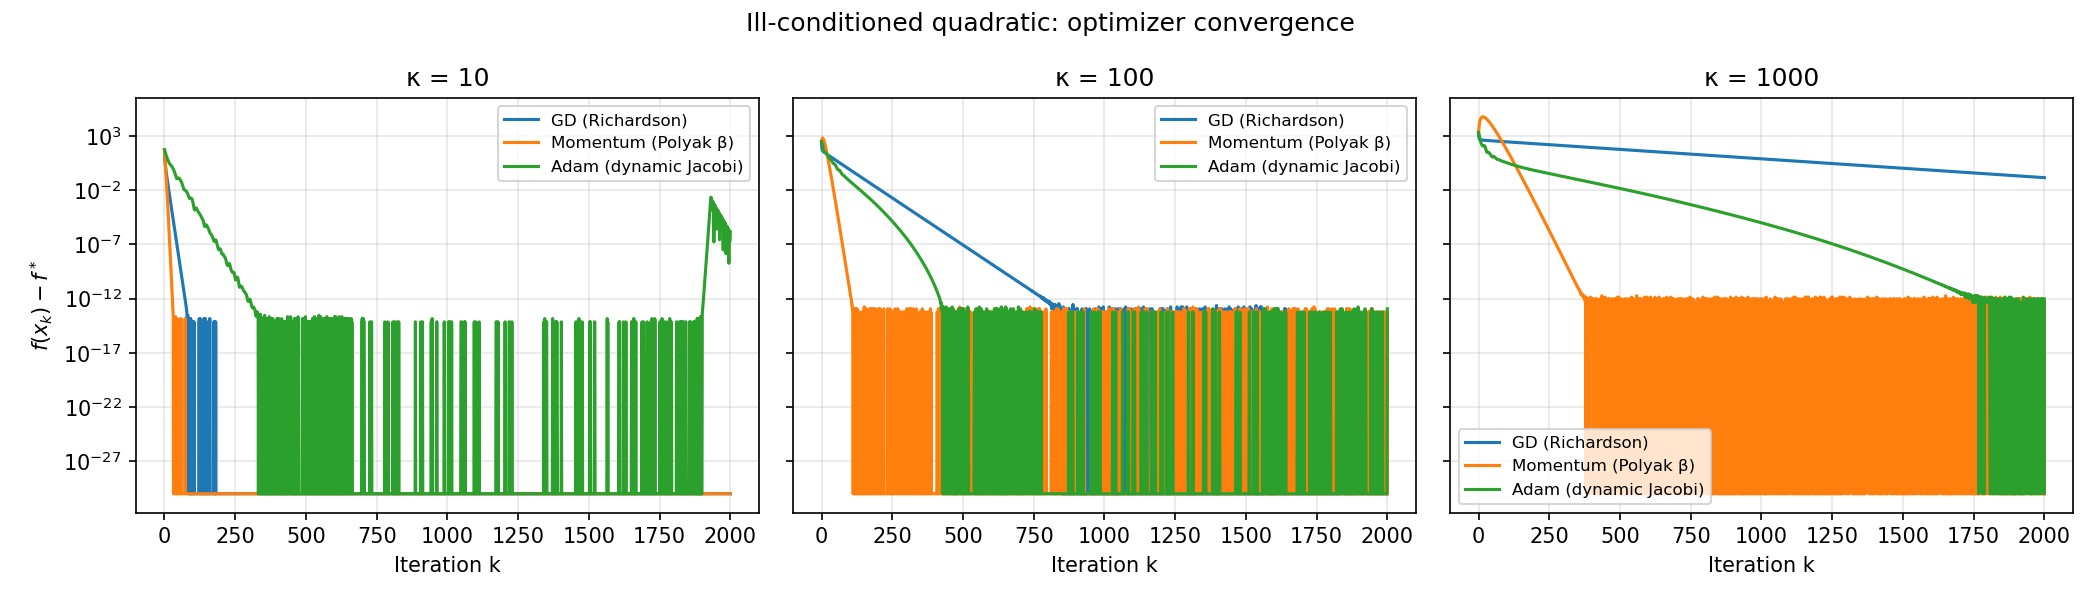
\includegraphics[width=0.95\linewidth]{exp1_convergence.png}%
  }{%
    \fbox{\parbox{0.8\linewidth}{\centering\vspace{2cm}图 exp1\vspace{2cm}}}%
  }
  \caption{$\kappa \in \{10, 100, 1000\}$ 下 GD / Heavy-ball / Adam 收敛曲线（实验 1）}
  \label{fig:exp1}
\end{figure}

\medskip
\noindent\textbf{图 25（exp25，主结果）}\quad
在 $\kappa = 100$、200 步的设置下，Heavy-ball 与 Chebyshev 半迭代的定常极限关系得到验证：左图两者末段 $f - f^*$ 曲线几乎完全重合，末 50 步最大差距为 $1.7 \times 10^{-13}$。

\begin{figure}[H]
  \centering
  \IfFileExists{../figures/exp25_hb_chebyshev.png}{%
    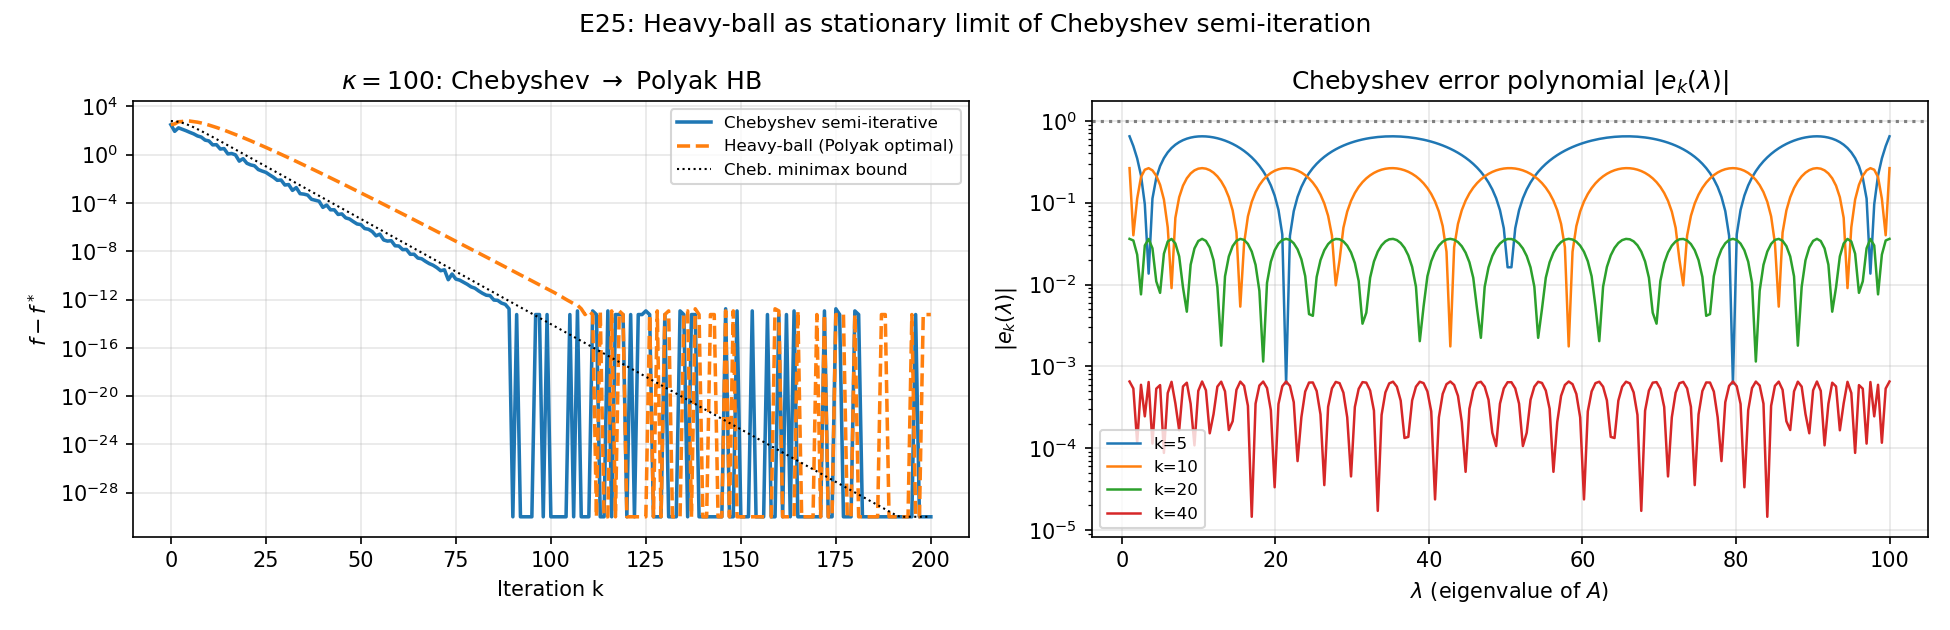
\includegraphics[width=0.95\linewidth]{exp25_hb_chebyshev.png}%
  }{%
    \fbox{\parbox{0.8\linewidth}{\centering\vspace{2cm}图 exp25\vspace{2cm}}}%
  }
  \caption{Heavy-ball 与 Chebyshev 半迭代的定常极限关系（实验 25）}
  \label{fig:exp25}
\end{figure}

\medskip
\noindent\textbf{图 26（exp26，Adam 2-极限环）}\quad
四组超参对照中，第 2 组形成清晰的 2-极限环 $\{0.025,\,-0.025\}$，是 Bock \& Wei{\ss} (2022) 理论的直接数值复现。

\begin{figure}[H]
  \centering
  \IfFileExists{../figures/exp26_adam_limit_cycle.png}{%
    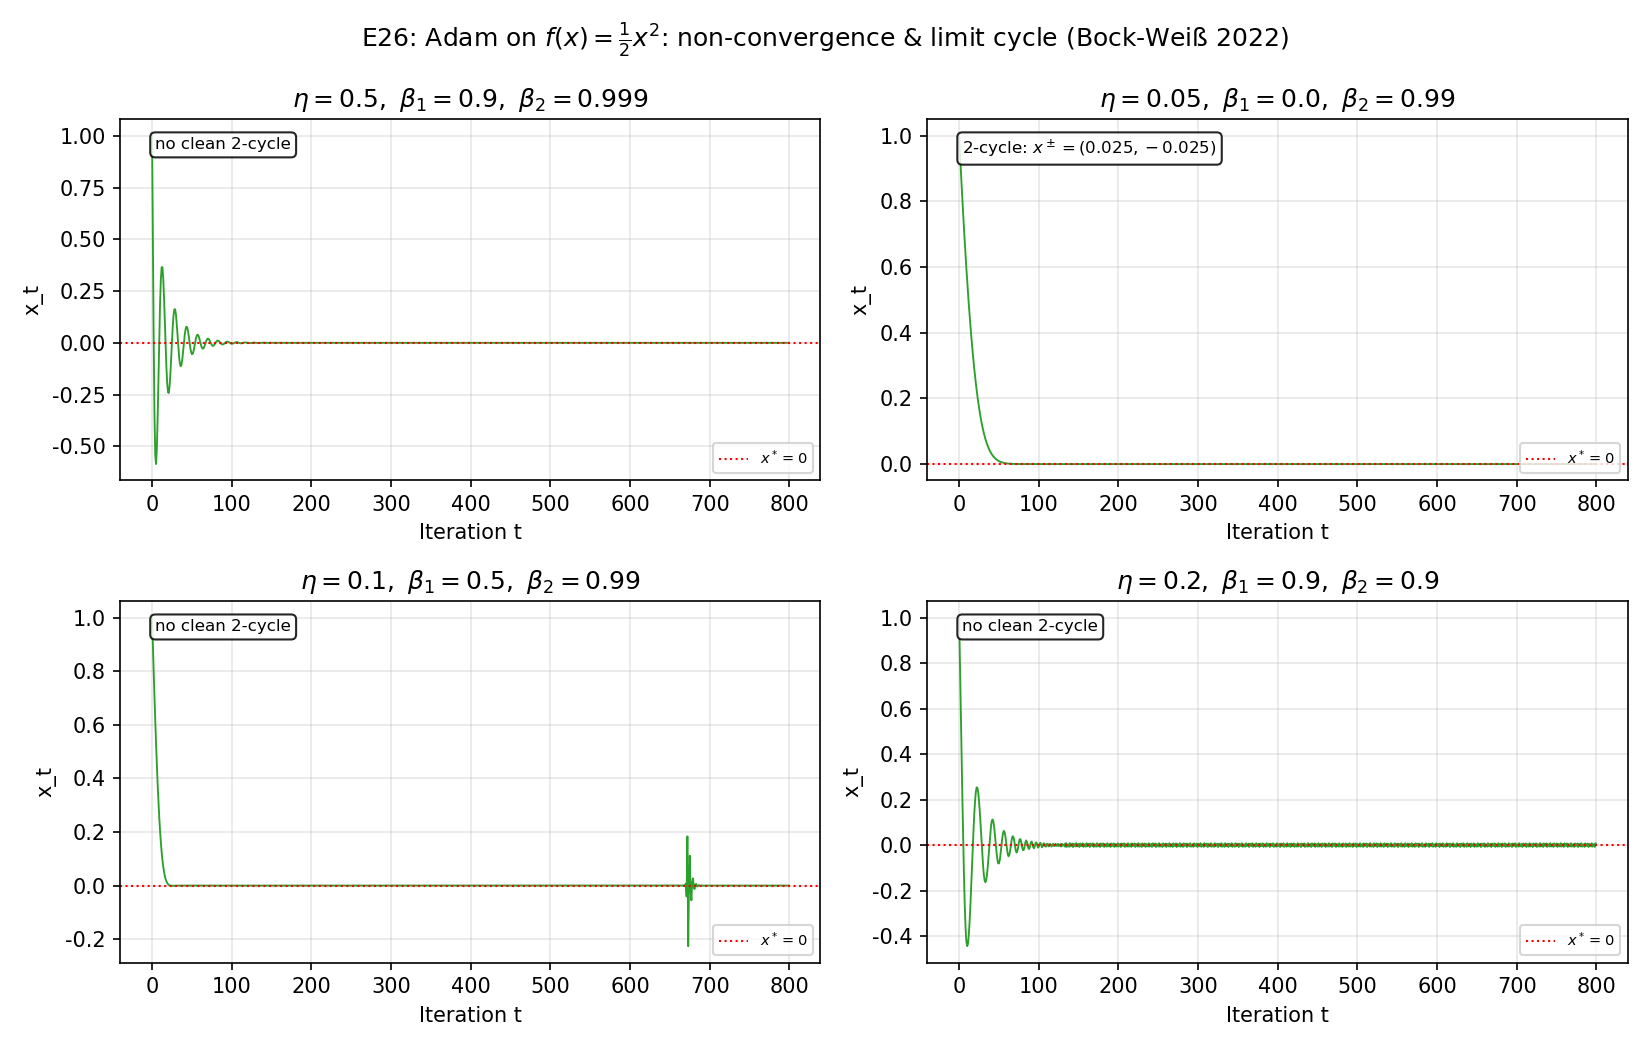
\includegraphics[width=0.9\linewidth]{exp26_adam_limit_cycle.png}%
  }{%
    \fbox{\parbox{0.8\linewidth}{\centering\vspace{2cm}图 exp26\vspace{2cm}}}%
  }
  \caption{Adam 2-极限环的数值复现（实验 26）}
  \label{fig:exp26}
\end{figure}

\medskip
\noindent\textbf{图 28（exp28，Muon 的主场）}\quad
在谱范数 trust-region 损失 $\tfrac{1}{2}\|W-W^*\|_\sigma^2$ 上，5 个种子的 Muon 均单调下降到 $0.028\sim 0.037$ 的稳定带，表明其正交化方向与谱范数几何相匹配。本实验维度 $m\times n=12\times 8$、$W_0=0$、$60$ 步、Muon 取 $\eta=0.3$、$T_{\mathrm{ns}}=8$、$\beta=0$，$W^*$ 的生成分布与超参细节见 \S\ref{sec:ns-muon}。

\begin{figure}[H]
  \centering
  \IfFileExists{../figures/exp28_muon_trust_region.png}{%
    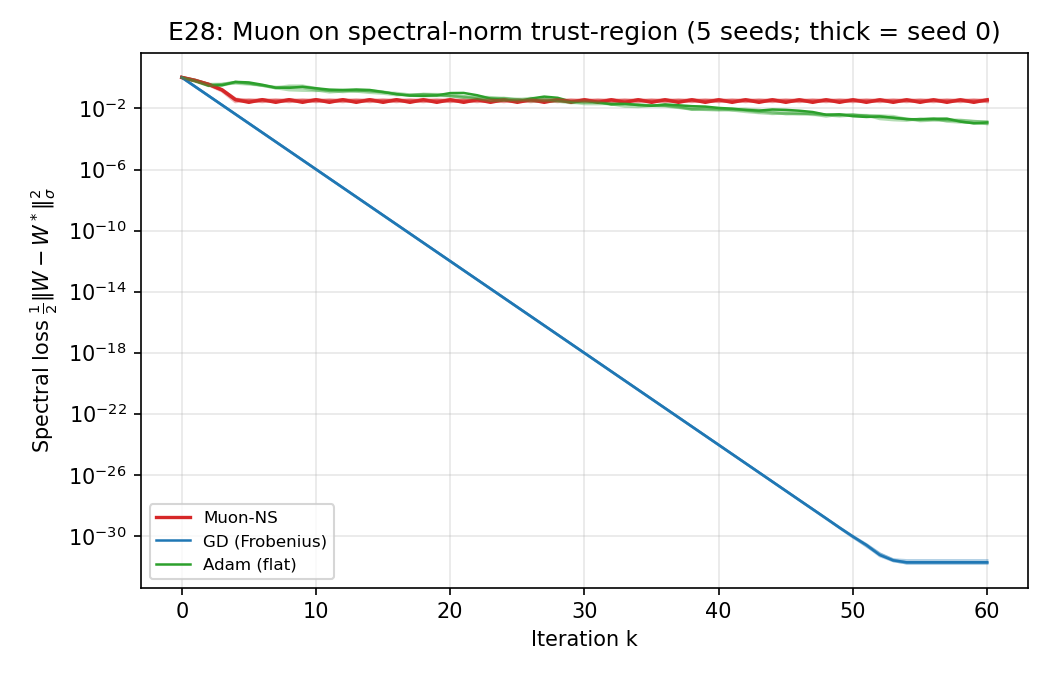
\includegraphics[width=0.9\linewidth]{exp28_muon_trust_region.png}%
  }{%
    \fbox{\parbox{0.8\linewidth}{\centering\vspace{2cm}图 exp28\vspace{2cm}}}%
  }
  \caption{Muon 在谱范数 trust-region 损失上的表现（实验 28）}
  \label{fig:exp28}
\end{figure}

\medskip\noindent\textbf{读图说明（为何 GD 曲线更低、更快？）}\quad
初值统一取 $W_0=0$ 时，Frobenius 梯度 $\nabla f(0)=0-W^*=-W^*$，GD 沿 $W^*$ 方向直线推进，对本实验随机生成的 $W^*$ 往往可将谱范数损失压至 $10^{-32}$ 量级（exp28 五种子的 GD 终值均 $\sim 10^{-32}$）。这是\textbf{初值与梯度形式的巧合}，并不表示 Muon 的全局最优性弱于 GD。

Muon 每步对 $g_k=W_k-W^*$ 做 Newton--Schulz 正交化，得到的是定理~\ref{thm:muon-tr} 中\textbf{谱范数 trust-region 线性子问题}的最速下降方向，而非全局最小化 $\tfrac{1}{2}\|W-W^*\|_\sigma^2$ 的精确最速下降；因此 Muon 会稳定停在约 $0.03$ 的平台，而不会像 GD 那样在 $W_0=0$ 时直达机器精度。本图要验证的是：Muon 在谱范数几何下\textbf{跨种子稳定下降}（与 exp12 右图 Frobenius 二次上 Muon 发散形成对照），而非与 GD 比拼最终精度。

\subsection{真实数据上的全连接层训练（实验 31）}
\label{sec:exp31}

前述实验均在合成的二次/标量算例上进行，便于与谱半径、收敛盆等理论量逐项对齐。为检验矩阵正交化预条件在\textbf{真实参数层}上的可用性，实验 31 在 scikit-learn 自带的手写数字数据集 \texttt{digits}（$8\times 8$ 灰度，共 $1797$ 张、$10$ 类）上训练一个单隐层全连接网络
\[
  x\in\mathbb{R}^{64}\ \xrightarrow{\,W_1\in\mathbb{R}^{64\times 32}\,}\ \mathrm{ReLU}\ \xrightarrow{\,W_2\in\mathbb{R}^{32\times 10}\,}\ \mathrm{softmax},
\]
以交叉熵为损失。两个权重 $W_1,W_2$ 都是矩阵参数层，正是 Muon 的作用对象：Muon 对每个权重的梯度矩阵做 $T_{\mathrm{ns}}=5$ 步 Newton--Schulz 正交化（动量 $\beta=0.9$）后更新，偏置等向量参数退化为带动量的一阶更新。对照方法为带动量 SGD 与 Adam。特征按训练集统计量标准化，数据按 $70\%/30\%$ 划分为 $1258$ 训练 / $539$ 测试，整批（full-batch）训练 $60$ 个 epoch，跨 $5$ 个随机种子。

三种方法在该真实任务上均稳定收敛，测试准确率高度接近：SGD 达 $0.961\pm 0.006$，Adam 达 $0.959\pm 0.006$，Muon 达 $0.961\pm 0.005$（峰值 $0.964$，三者中最高）。值得注意的是 Muon 的训练交叉熵下降到 $\sim 4\times 10^{-5}$，明显低于 Adam（$\sim 5\times 10^{-3}$）与 SGD（$\sim 9\times 10^{-3}$），说明其逐层正交化的更新方向在真实矩阵参数上同样能高效拟合训练数据，并保持与主流优化器相当的泛化。这与谱范数 trust-region 的解释一致：当被优化对象本身是矩阵参数层时，Muon 的正交化预条件给出了与 Adam/ SGD 不同但同样有效的下降几何。

\begin{figure}[H]
  \centering
  \IfFileExists{../figures/exp31_mlp_digits.png}{%
    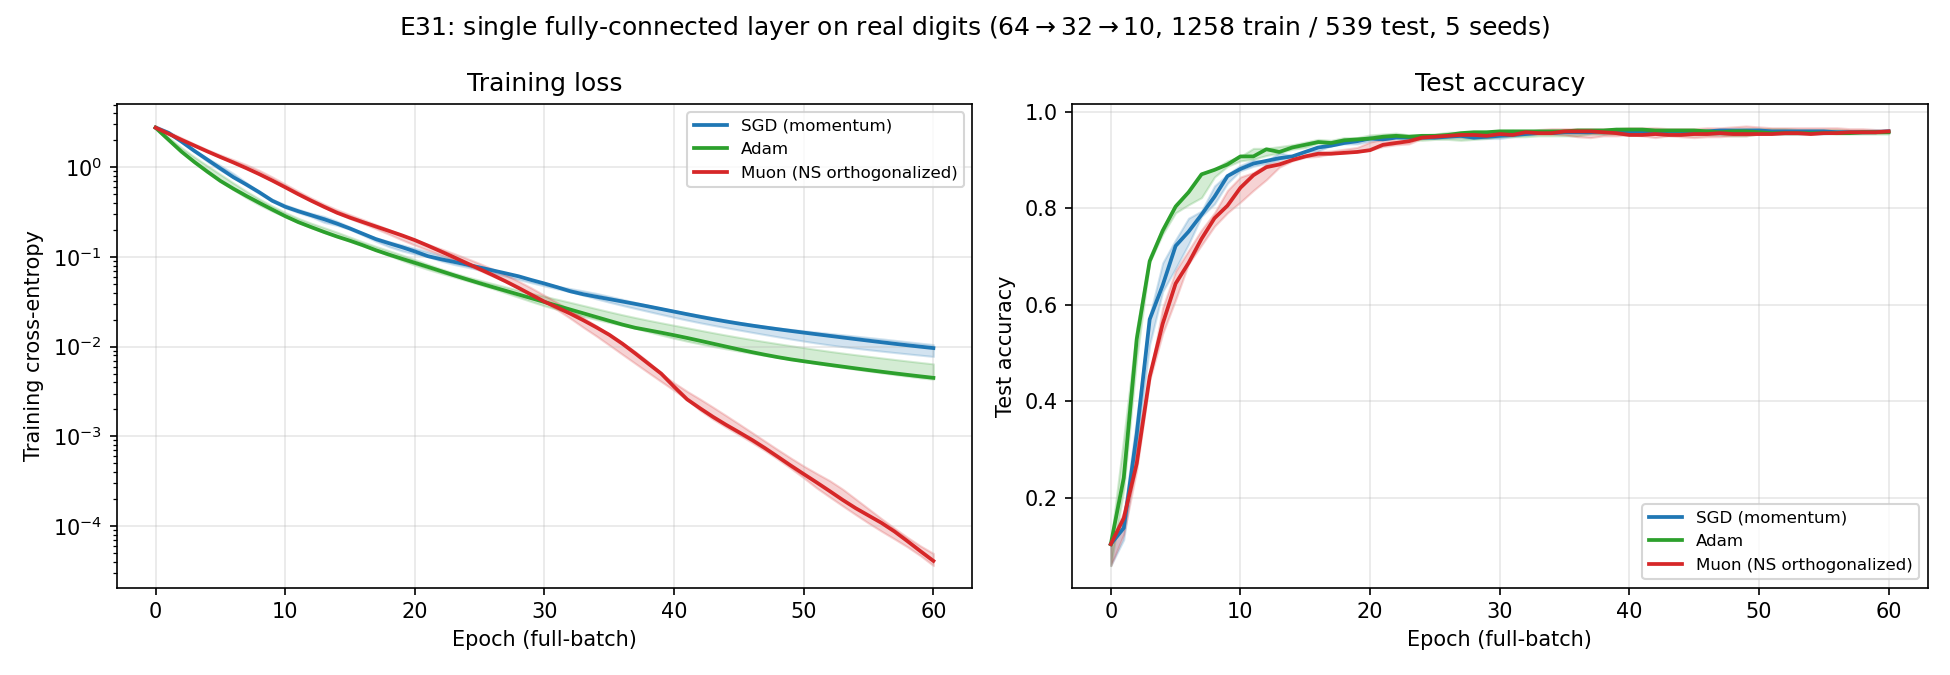
\includegraphics[width=0.95\linewidth]{exp31_mlp_digits.png}%
  }{%
    \fbox{\parbox{0.8\linewidth}{\centering\vspace{2cm}图 exp31\vspace{2cm}}}%
  }
  \caption{真实数据（\texttt{digits}）上单隐层 MLP 的训练损失（左）与测试准确率（右），SGD / Adam / Muon 跨 5 种子的中位数与四分位带（实验 31）}
  \label{fig:exp31}
\end{figure}

\section{结论}
\label{sec:conclusion}

\begin{enumerate}[nosep]
  \item \textbf{统一模板} $x_{k+1} = x_k - P_k g_k$ 把 GD（Richardson）、Heavy-ball（谱加速）、Adam（动态 Jacobi）、Sophia（对角 Hessian）、Muon（极分解）放在同一数值迭代框架下。
  \item \textbf{谱半径分析}精确预测二次问题上的收敛率：GD $\rho^* = (\kappa-1)/(\kappa+1)$、Polyak HB $\rho^* = (\sqrt\kappa-1)/(\sqrt\kappa+1)$；实验 2 直接验证。
  \item \textbf{HB 是 Chebyshev 半迭代的定常极限}（定理~\ref{thm:hb-cheb} + 实验 25）：两者末段 gap 差距 $1.7 \times 10^{-13}$。
  \item \textbf{Newton--Schulz 二次收敛}有干净的递推 \eqref{eq:ns-error}，收敛盆 $(0, \sqrt 3)$ 由实验 30 在 100 个初值上直接观察证实。
  \item \textbf{Muon 的真本质}是谱范数 trust-region 线性子问题的最速下降方向（定理~\ref{thm:muon-tr}）；它在谱范数恢复目标上稳定下降，在 Frobenius 损失上不下降是几何错配。
  \item \textbf{Adam 2-极限环}（实验 26）复现 Bock \& Wei{\ss} (2022)：即使最简凸 $f(x) = x^2/2$ 上 Adam 也可能不收敛。
  \item \textbf{NAG $\leftrightarrow$ ODE}（实验 29）：AVD-ODE 的 RK4 解与离散 NAG 在 $t = \sqrt\eta k$ 下呈现相近轨迹。
\end{enumerate}

\section{作者分工与贡献}

本报告由两人合作完成，具体分工如下：

\begin{table}[htbp]
  \centering
  \caption{作者分工与贡献比例}
  \label{tab:contribution}
  \begin{tabular}{@{}lll@{}}
    \toprule
    作者 & 学号 & 主要贡献 \\
    \midrule
    赵泽霖 & 2023010848 & 理论推导、定理证明、Newton--Schulz/Muon 章节撰写、报告整体架构 \\
    史云天 & 2023010836 & 数值实验设计与实现、代码开发、图表生成、实验章节撰写 \\
    \bottomrule
  \end{tabular}
\end{table}

\noindent 贡献比例：赵泽霖 50\%，史云天 50\%。


\bibliographystyle{plainnat}
\bibliography{references}

\appendix
% \section{代码与 $P_k$ 对照表}
\label{app:code}

\begin{table}[htbp]
  \centering
  \caption{主要源代码文件}
  \small
  \begin{tabular}{@{}ll@{}}
    \toprule
    文件 & 内容 \\
    \midrule
    \texttt{src/quadratic.py} & 病态二次构造、目标、梯度 \\
    \texttt{src/optimizers.py} & gd / momentum / nesterov / adam / adamw / sophia / jacobi \\
    \texttt{src/newton\_schulz.py} & 标准 NS + 五次多项式 Higham \\
    \texttt{src/chebyshev.py} & Chebyshev 半迭代 + HB-Polyak 形式 \\
    \texttt{src/spectral\_trust\_region.py} & 谱范数恢复 + Muon/GD/Adam 对照 \\
    \texttt{src/adam\_limit\_cycle.py} & 标量 Adam + 2-极限环检测 \\
    \texttt{src/ode\_integrators.py} & 梯度流 / AVD-ODE 的 RK4 \\
    \texttt{experiments/run\_all.py} & 实验 1--10 + 入口 \\
    \texttt{experiments/extended\_experiments.py} & 实验 11--30 \\
    \texttt{tests/test\_*.py} & 14 项回归测试 \\
    \bottomrule
  \end{tabular}
\end{table}

\begin{table}[htbp]
  \centering
  \caption{$P_k$ 形态与优化器对照}
  \small
  \begin{tabular}{@{}lll@{}}
    \toprule
    $P_k$ 形态 & 优化器 & 代码标签 \\
    \midrule
    $\eta I$ & GD & \texttt{gd} \\
    二阶状态 + $\eta I$ & Polyak HB & \texttt{momentum} \\
    二阶状态 + lookahead & Nesterov & \texttt{nesterov} \\
    $\eta\,\mathrm{diag}(\sqrt{\hat v_k})^{-1}$ & Adam & \texttt{adam} \\
    Newton--Schulz 正交化 & Muon & \texttt{muon\_direction} \\
    Chebyshev 时变 $\omega_k$ & Chebyshev 半迭代 & \texttt{chebyshev\_semi\_iterative} \\
    \bottomrule
  \end{tabular}
\end{table}
  % 附录 A：代码与 P_k 对照表（暂注释，需要时恢复）
\section{实验数值摘要（精选）}
\label{app:data}

数据来源：\texttt{data/experiment\_results.json}。完整版见 \texttt{report/appendix\_auto.md}。

\subsection{实验 1：达到 $10^{-6}$ 的迭代步数}
\label{app:exp1}

\noindent 下表给出不同条件数下各方法达到 $10^{-6}$ 精度所需的迭代步数。
\begin{center}
  \vspace{0.5em}
  \begin{tabular}{@{}cccc@{}}
    \toprule
    $\kappa$ & GD & Polyak HB & Adam \\
    \midrule
    10   & 39  & 17  & 162 \\
    100  & 439 & 68  & 288 \\
    1000 & --- ($>$2000) & 256 & 1133 \\
    \bottomrule
  \end{tabular}
  \vspace{0.5em}
\end{center}

\subsection{实验 12：Muon 在两种损失上}
\label{app:exp12}

\noindent Muon 在谱范数损失与 Frobenius 矩阵二次上的最终损失对比如下。
\begin{center}
  \vspace{0.5em}
  \begin{tabular}{@{}lccc@{}}
    \toprule
    目标 & Muon-NS 最终 & GD 最终 & Adam 最终 \\
    \midrule
    谱范数损失 (80 步)      & 0.037   & $2.4\times 10^{-32}$ & $1.1\times 10^{-4}$ \\
    Frobenius 二次 (400 步) & 63266   & 51.4                 & --- \\
    \bottomrule
  \end{tabular}
  \vspace{0.5em}
\end{center}

\subsection{实验 25：HB $\equiv$ Chebyshev 半迭代}
\label{app:exp25}

\noindent Heavy-ball 与 Chebyshev 半迭代末段数值对比如下。
\begin{center}
  \vspace{0.5em}
  \begin{tabular}{@{}lc@{}}
    \toprule
    量 & 值 \\
    \midrule
    200 步后 $f - f^*$（HB）   & $10^{-30}$ \\
    200 步后 $f - f^*$（Cheb） & $10^{-30}$ \\
    max gap diff（末 50 步）   & $1.7 \times 10^{-13}$ \\
    \bottomrule
  \end{tabular}
  \vspace{0.5em}
\end{center}

\subsection{实验 30：Newton--Schulz 收敛盆}
\label{app:exp30}

\noindent 理论收敛盆上界 $\sqrt{3} \approx 1.7321$。在 100 个 $\sigma_0 \in [0.05, 2.5]$ 中，\textbf{11 个发散}，且全部满足 $\sigma_0 > \sqrt{3}$，与定理~\ref{thm:ns} 的预言完全一致。

\section{完整证明}
\label{app:proofs}

\subsection{定理~\ref{thm:gd} 的证明（GD 线性收敛）}

设 $A = Q\Lambda Q^\top$，$0 < \mu \le \lambda_i \le L$。GD 更新 $x_{k+1} = x_k - \eta(A x_k - b)$，误差 $e_k = x_k - x^*$ 满足 $e_{k+1} = (I - \eta A) e_k$。在特征基下各模态衰减为 $|1 - \eta\lambda_i|$，故
\[
  \|e_{k+1}\|_2 \le \max_i |1 - \eta\lambda_i| \cdot \|e_k\|_2 = \rho(\eta)\,\|e_k\|_2.
\]
$\rho(\eta) = \max\{|1 - \eta\mu|, |1 - \eta L|\}$ 在 $\eta = 2/(\mu+L)$ 处取最小值 $\rho^* = (\kappa-1)/(\kappa+1)$。$\square$

\subsection{定理~\ref{thm:hb} 的证明（Polyak 最优 Heavy-ball）}

在特征基下，Heavy-ball 对每个模态 $\lambda$ 给出 $2\times 2$ 矩阵 $T(\lambda)$，特征方程 $z^2 - (1 - \eta\lambda + \beta) z + \beta = 0$。最优情形要求所有 $\lambda\in[\mu,L]$ 满足 $(1 - \eta\lambda + \beta)^2 \le 4\beta$，端点同时取等：
\[
  1 - \eta\mu + \beta = 2\sqrt\beta,\quad -(1 - \eta L + \beta) = 2\sqrt\beta.
\]
解得 $\beta^* = \bigl(\frac{\sqrt L - \sqrt\mu}{\sqrt L + \sqrt\mu}\bigr)^2$，$\rho^* = (\sqrt\kappa - 1)/(\sqrt\kappa + 1)$，$\eta^* = 4/(\sqrt L + \sqrt\mu)^2$。$\square$

\subsection{定理~\ref{thm:hb-cheb} 的证明（HB 是 Chebyshev 半迭代的定常极限）}

Chebyshev 半迭代（Hageman--Young 形式）：
\[
  \omega_1 = \frac{1}{1 - \sigma^2/2},\quad
  \omega_{k+1} = \frac{1}{1 - \sigma^2 \omega_k / 4},\quad
  x_{k+1} = \omega_{k+1}\left(\frac{r_k}{d} + x_k - x_{k-1}\right) + x_{k-1},
\]
其中 $d = (L+\mu)/2$，$\sigma = (L-\mu)/(L+\mu)$。令 $\omega_k \to \omega_\infty$，不动点方程给出 $\omega_\infty = 2/(1 + \sqrt{1-\sigma^2})$。可验证 $\eta_\infty = \omega_\infty/d = \eta^*$、$\beta_\infty = \omega_\infty - 1 = \beta^*$，故 Chebyshev 在系数收敛后退化为 Polyak 最优 Heavy-ball。实验 25 末段 gap $1.7\times 10^{-13}$ 与该解释一致。$\square$

\subsection{命题~\ref{prop:adam-jacobi} 的证明}

$\beta_1 = 0$ 时 $\hat m_k = g_k$；$v_k$ 趋于 $\mathbb{E}[g \odot g]$。对二次问题 $g(x) = A(x - x^*)$，当 $A$ 对角且 $\Sigma \propto I$ 时 $\mathbb{E}[g \odot g]\propto \mathrm{diag}(A)^2$，故 $P_k \approx \eta\,\mathrm{diag}(A)^{-1}$，恰为 Jacobi 预条件器。$\square$

\subsection{定理~\ref{thm:ns} 与命题~\ref{prop:basin} 的证明（Newton--Schulz 收敛盆）}

定理~\ref{thm:ns} 的误差递推 $E_{k+1}=-\tfrac14 E_k^2(3I-E_k)$ 的推导见正文 \S\ref{sec:ns-muon}。这里补全收敛盆 $(0,\sqrt3)$ 的严格证明。

\textbf{第一步：约简到标量映射。}\quad 迭代 \eqref{eq:ns} 只经 $X_k^\top X_k$ 作用于 $X_k$。设 $X_k=P_k\Sigma_k Q_k^\top$ 为 SVD，则 $X_k^\top X_k=Q_k\Sigma_k^2 Q_k^\top$，代入得
\[
  X_{k+1}=\tfrac12 P_k\Sigma_k(3I-\Sigma_k^2)Q_k^\top=P_k\,\varphi(\Sigma_k)\,Q_k^\top,
  \qquad \varphi(\sigma)=\tfrac12\sigma(3-\sigma^2).
\]
故奇异向量 $P_k\equiv P_0,\ Q_k\equiv Q_0$ 不随迭代改变，全部动力学集中在奇异值上：$\sigma^{(i)}_{k+1}=\varphi(\sigma^{(i)}_k)$，各分量解耦。$X_k\to U=P_0 Q_0^\top$（极分解正交因子）当且仅当所有 $\sigma^{(i)}_k\to1$。

\textbf{第二步：标量映射 $\varphi$ 在 $(0,\sqrt3)$ 上收敛到 $1$。}\quad
不动点方程 $\varphi(\sigma)=\sigma$ 化为 $\sigma(1-\sigma^2)=0$，正实轴上唯一非零不动点为 $\sigma^*=1$。导数 $\varphi'(\sigma)=\tfrac32(1-\sigma^2)$，于是 $\varphi'(1)=0$，$\sigma^*=1$ 为超吸引不动点。

\emph{(a) $\sigma\in(0,1]$。}\quad 此区间上 $\varphi'(\sigma)\ge0$，$\varphi$ 单调不减，且 $\varphi(0)=0,\varphi(1)=1$，故 $\varphi$ 自映 $(0,1]$。差式 $\varphi(\sigma)-\sigma=\tfrac12\sigma(1-\sigma^2)>0$（$\sigma\in(0,1)$），故迭代序列单调递增、上有界于 $1$，从而收敛，且极限为该区间唯一不动点 $1$。

\emph{(b) $\sigma\in(1,\sqrt3)$。}\quad 此区间上 $\varphi'(\sigma)<0$，$\varphi$ 单调递减，$\varphi(1)=1,\ \varphi(\sqrt3)=0$，故 $\varphi\bigl((1,\sqrt3)\bigr)=(0,1)$。任何此区间内的 $\sigma_0$ 一步后进入 $(0,1)$，回到情形 (a)，单调递增收敛到 $1$。

合并 (a)(b)：$(0,\sqrt3)$ 整体是 $\sigma^*=1$ 的吸引盆，且迭代恒保持在 $(0,\sqrt3)$ 内（不会逃逸）。

\textbf{第三步：二次收敛率。}\quad 令 $e_k=\sigma_k-1$。在 $\sigma=1$ 处 Taylor 展开 $\varphi(\sigma)=\varphi(1)+\varphi'(1)(\sigma-1)+\tfrac12\varphi''(1)(\sigma-1)^2+\tfrac16\varphi'''(1)(\sigma-1)^3$，其中 $\varphi'(1)=0,\ \varphi''(\sigma)=-3\sigma\Rightarrow\varphi''(1)=-3,\ \varphi'''(\sigma)=-3\Rightarrow\varphi'''(1)=-3$，得
\[
  e_{k+1}=-\tfrac32 e_k^2-\tfrac12 e_k^3,
  \qquad |e_{k+1}|\le\tfrac32|e_k|^2\ \ (|e_k|\le1).
\]
这与正文矩阵递推 $E_{k+1}=-\tfrac14E_k^2(3I-E_k)$ 在标量化（$E_k=\sigma_k^2-1$）下完全一致：$\sigma_k^2-1\approx2e_k$ 时两式同阶。

\textbf{第四步：发散侧。}\quad 若 $\sigma_0>\sqrt3$，则 $3-\sigma_0^2<0$，故 $\sigma_1=\tfrac12\sigma_0(3-\sigma_0^2)<0$；当 $|\sigma|$ 较大时 $\varphi(\sigma)\approx-\tfrac12\sigma^3$，$|\sigma_k|$ 以三次速度发散。这解释了实验 30 中 $\sigma_0>\sqrt3$ 的 $11$ 个初值全部发散。$\square$

\subsection{定理~\ref{thm:muon-tr} 的证明}

定理~\ref{thm:muon-tr} 的证明见正文 \S\ref{sec:ns-muon}，基于 von Neumann 迹不等式取等条件。


\end{document}
